% IJTAF submission copy of ../weakorder_paper_clean.tex, converted from the
% SIFIN copy ../sifin/p4_sifin.tex. Body text and thebibliography verbatim;
% only the class/front-matter block is converted, to the World Scientific
% class ws-ijtaf.cls v1.5g (2026/07/02) in this folder, obtained from IJTAF's
% own submission-guidelines page. The class loads amsfonts/amssymb/amsmath/
% graphicx/natbib itself and predefines theorem/corollary/lemma/proposition/
% definition/example/remark (numbered by section) -- so the SIAM-era explicit
% amssymb load and the \newsiamremark declaration are both dropped here.
\documentclass{ws-ijtaf}

\usepackage[utf8]{inputenc}
\usepackage[T1]{fontenc}
\usepackage{mathtools}
\usepackage{booktabs}
\usepackage{xcolor}
\usepackage[verbose,hypertexnames=false]{hyperref}
\hypersetup{colorlinks=false,allbordercolors=blue,pdfborderstyle={/S/U/W 1}}

\begin{document}
% THEORY vs MEASURED (for the reframe; rough-Bergomi theory, rough-Heston measurement)
%   left-point (3H+1/2)^1 : H=0.05 -> 0.65 | H=0.10 -> 0.80 | H=0.20 -> 1.00  [Gassiat; FSW optimal]
%   hybrid weights H+1/2  : H=0.05 -> 0.55 | H=0.10 -> 0.60 | H=0.20 -> 0.70  [Gassiat; BFN]
%   measured alpha (this paper): H=0.05 -> 0.74 | H=0.10 -> unresolved | H=0.20 -> ~1

\markboth{M. Lumor}{Weak Order of a Direct Rough Heston Discretisation}

%%%%%%%%%%%%%%%%%%%%% Publisher's Area please ignore %%%%%%%%%%%%%%%
\catchline{}{}{}{}{}
%%%%%%%%%%%%%%%%%%%%%%%%%%%%%%%%%%%%%%%%%%%%%%%%%%%%%%%%%%%%%%%%%%%%

\title{WEAK CONVERGENCE IS FASTER THAN STRONG:\\
THE WEAK ORDER OF A DIRECT ROUGH HESTON DISCRETISATION,\\
MEASURED AGAINST GAUSSIAN-VOLATILITY THEORY}

\author{MICHAEL LUMOR}

\address{School of Science, Engineering and Environment, University of Salford\\
Salford, United Kingdom\\
\email{m.lumor@edu.salford.ac.uk}}

\maketitle

\begin{history}
\received{(Day Month Year)}
\revised{(Day Month Year)}
\end{history}

\begin{abstract}
The hybrid scheme of Bennedsen, Lunde and Pakkanen is the standard simulator for
rough stochastic volatility, and its \emph{strong} (pathwise) convergence order is
the Hurst exponent $H$---so at the empirically relevant $H\approx 0.1$, pathwise
accuracy nearly stalls. Whether \emph{prices} stall too is a question about the
weak order $\alpha$, and there the theory is model-specific. For
Gaussian-volatility models, recent work establishes weak rates of
$(3H+\tfrac12)\wedge 1$ for left-point discretisation---proven optimal, with a
phase transition at $H=\tfrac16$---and $H+\tfrac12$ for the weighted hybrid
scheme. No such result covers rough Heston, whose square-root Volterra dynamics
fall outside these theorems. We measure the weak order of the direct hybrid-type
discretisation of rough Heston against a simulation-free characteristic-function
reference, committing before measurement to the prediction $\alpha>H$.
Romano--Touzi conditioning makes estimation feasible and is bias-preserving by
construction. We find $\alpha\gg H$ throughout: $\alpha\approx 1$ at $H=0.20$,
with a genuine penalty only at the rough extreme, $\alpha\approx 0.74$ at
$H=0.05$---reproducing, in a model the theorems do not cover, the qualitative
phase structure they prove. The intermediate $H=0.10$ is not resolvable at the
explicit scheme's $O(n^2)$ cost; a multifactor Markovian lift cannot settle it,
since its noise approximation perturbs the measured rate itself.
\end{abstract}

\keywords{Rough volatility; rough Heston; weak convergence; discretisation error;
Monte Carlo.}

\ccode{AMS Subject Classification: 60H35, 65C30, 91G60}

\section{Introduction}\label{sec:intro}

Rough stochastic volatility models---in which log-volatility is driven by a
fractional process with Hurst exponent $H\approx 0.1$---reproduce the steep
short-maturity implied-volatility skew that classical diffusive models miss, and
have become a central object of study in quantitative finance since the work of
Gatheral, Jaisson and Rosenbaum~\citeyearpar{gjr2018}. Pricing under these models is not analytically
tractable in general and rests on Monte Carlo simulation of the underlying rough
Volterra dynamics~\citep{bfg2016}. The standard simulator is the \emph{hybrid scheme} of
Bennedsen, Lunde and Pakkanen~\citeyearpar{blp2017} (henceforth BLP), which discretises the
$(t-s)^{H-1/2}$ kernel on a refining time grid.

A discretisation scheme is characterised by two convergence orders, and they
measure different things. The \emph{strong} order controls the pathwise
$L^2$ error $\big(\mathbb{E}\,|X_T^\Delta - X_T|^2\big)^{1/2}$; the \emph{weak}
order $\alpha$ controls the error in expectations of functionals,
$\big|\mathbb{E}\,g(X_T^\Delta) - \mathbb{E}\,g(X_T)\big| = O(\Delta t^{\alpha})$.
For pricing, it is the \emph{weak} order that matters: an option price is an
expectation, and the bias in a Monte Carlo price decays at the weak rate, not the
strong rate. For classical It\^o diffusions under an Euler scheme the two orders are
$\tfrac12$ (strong) and $1$ (weak)---weak convergence is faster, because the
pathwise fluctuations that limit the strong error largely cancel in expectation.

For the BLP hybrid scheme the strong order is known: it is $H$, so that the
$L^2$ error decays as $O(n^{-H})$ in the number of steps $n$. This is a result of
BLP, and it is tight---the pathwise bound is achieved with equality, which can be
seen empirically through the Giles~\citeyearpar{giles2008} level-variance decay rate $\beta = 2H$ that the
strong order implies.\footnote{This corroboration is established separately in the
\texttt{RoughVolLab} programme of which the present work is a part; the measured
$\beta$ tracks $2H$ across $H\in\{0.05,0.10,0.20,0.35\}$ with equality.} The
practical consequence is stark: at the empirically relevant $H\approx 0.1$, the
strong rate is $O(n^{-0.1})$---roughness throttles pathwise convergence almost to a
standstill.

How fast prices converge is a question the strong order cannot answer, and for rough
volatility the weak-rate theory that does answer it is model-specific. For
\emph{Gaussian-volatility} models---rough Bergomi and its relatives, where the variance is a
(function of a) Gaussian Volterra process---the weak rate of the left-point discretisation is
$(3H+\tfrac12)\wedge 1$: established by Gassiat~\citeyearpar{gassiat2023} for fBm integrands and
cubic test functions, extended and proven \emph{optimal}, with a matching lower bound and a
phase transition at $H=\tfrac16$, by Friz, Salkeld and Wagenhofer~\citeyearpar{fsw2025}, and
recovered through path-dependent PDEs by Bonesini, Jacquier and Pannier~\citeyearpar{bjp2023}; the
weighted hybrid scheme attains $H+\tfrac12$~\citep{gassiat2023,bfn2022}, and Bayer, Hall and
Tempone~\citeyearpar{bht2023} treat option pricing under linear rough volatility. Results in
the Gaussian and nonsingular classes continue to appear: Alfonsi and Kebaier obtain
rates for rough Stein--Stein-type (mean-reverting Gaussian) volatility via
integrated-kernel Euler schemes~\citeyearpar{ak2026}, and Bras and Fukasawa treat nonsingular
stochastic Volterra equations~\citeyearpar{bf2025}. None of these
theorems covers the \emph{rough Heston} model: its variance is a square-root Volterra
process---non-Gaussian, with a diffusion coefficient that is neither linear nor smooth at the
origin---and it is rough Heston that this paper discretises. What is known there concerns
Markovian approximations: Bayer and Breneis bound the weak error of the approximation by the
$L^1$ kernel error~\citeyearpar{bb2023} and report second-order weak convergence for a weak
simulation scheme built on it, alongside a numerically observed rate of one for Gatheral's
HQE scheme~\citep{bb2024}---schemes, in both cases, other than the direct discretisation.
\textbf{The question this paper answers is empirical: what weak rate does the direct
hybrid-type discretisation of rough Heston exhibit, and does it match the phase structure
the Gaussian-volatility theory proves?}

Following the discipline of committing a falsifiable prediction before measurement,
we state our hypothesis up front: we predict $\alpha > H$ (the weak rate is faster
than the strong rate, as in the classical case), and we expect $\alpha\approx 1$
for a smooth payoff if roughness does not bottleneck the bias. Three outcomes are
possible, and we pre-specify all three as reportable: $\alpha\approx 1$ (the
classical weak order survives---roughness does not throttle pricing);
$H < \alpha < 1$ (a quantified roughness penalty on the weak rate); or
$\alpha\approx H$ (roughness throttles the weak rate too---the strong-order
pessimism carries, contradicting the classical expectation).

Measuring a weak order is harder than it sounds, for two reasons that organise the
methodology of this paper. First, \emph{circularity}: the weak error is the bias of
a simulated price against the \emph{true} price, and the true price is not known in
closed form for rough volatility. Comparing a coarse simulation against a fine
simulation measures self-consistency, not convergence to truth, and cannot validly
recover the order of the very scheme under test. We resolve this by pricing against
a \emph{simulation-free} reference: the rough-Heston characteristic function of El
Euch and Rosenbaum, evaluated through a fractional Riccati equation and Fourier
inversion. This reference is validated by its reduction, at $H=\tfrac12$, to the
classical Heston price, for which a closed form is available---so the reference is
anchored to a known answer before it is trusted at $H<\tfrac12$. Second,
\emph{signal-to-noise}: precisely because we predict $\alpha > H$, the bias decays
faster than the scale of the sampling error as the grid refines, so the measurable
window is confined to coarse-to-intermediate grids and fine grids are intrinsically
noise-dominated. Naive estimation of the bias against the reference cannot resolve
$\alpha$ at all; we recover it using Romano--Touzi~\citeyearpar{rt1997} conditional Monte Carlo, which
integrates the orthogonal asset Brownian motion out analytically and slashes the
sampling variance while preserving the discretisation bias.

Our central finding is that \textbf{the strong-order roughness pessimism does not
carry to the weak rate}. Across the tested range $H\in\{0.05,0.10,0.20\}$ we
measure $\alpha \gg H$---weak convergence is far faster than strong---with
$\alpha\approx 1$ at $H=0.20$, consistent with the classical weak order, and a
genuine but modest roughness penalty emerging only at the rough extreme, where
$\alpha\approx 0.74$ at $H=0.05$ (below $1$ at eight standard errors). This is,
qualitatively, the phase structure the Gaussian-volatility theory proves---the classical
rate above $H=\tfrac16$, a genuine sub-unit penalty below it---reproduced in a model the
theorems do not cover. Quantitatively, the sub-transition exponent sits somewhat above the
Gaussian-theory line: $0.74$--$0.77$ across fit windows against $3H+\tfrac12=0.65$, a gap
we report as an observation, not a refutation---the theorems do not apply to rough Heston,
and the fitted exponent is an effective rate over the measurable window. The
pricing accuracy of the hybrid scheme therefore survives roughness even in the
regime where its pathwise accuracy collapses. We report the boundary of the method
with equal care: an intermediate regime, $H=0.10$---where the Gaussian-theory target is
$0.80$---exhibits a pre-asymptotic
ambiguity that more sampling cannot resolve and that the $O(n^2)$ cost of the
explicit scheme prevents us from settling with finer grids. The natural remedy is a
multifactor Markovian lift, which replaces the singular convolution kernel by a sum
of exponentials and so reduces the per-step cost from $O(n)$ to $O(N)$ in the number
of factors, affording the finer grids the explicit scheme cannot reach. We construct
this lift and validate it against the same characteristic-function reference---and
arrive at a negative result: the lift cannot settle the borderline. To keep the
factor system at $O(Nn)$, the per-factor noise integrals are replaced by a common
effective increment---a rank-one approximation of the joint factor noise whose cost
saving is what makes the lift cheap; we show this approximation perturbs the weak rate
itself, by an amount that is independent of the number of factors and therefore not
removable by refining the kernel approximation. We characterise the failure mode
precisely and situate it against the Markovian-approximation results of Bayer and
Breneis~\citeyearpar{bb2023,bb2024}. The lift reproduces the strong rate and prices correctly, yet
measures a weak rate that is not the true one. So the $H=0.10$ borderline is not
merely unresolved but resolution-resistant by the natural method, and we characterise
exactly why.

The remainder of the paper is organised as follows.
Section~\ref{sec:scheme} fixes the model and the scheme and states the convergence
question precisely. Section~\ref{sec:method} develops the measurement framework:
the non-circular characteristic-function reference and its validation, the native
rough-Heston simulator, and the variance-reduced estimators.
Section~\ref{sec:results} reports the measured weak order.
Section~\ref{sec:lift} constructs the multifactor Markovian lift and establishes the
negative result---that its noise approximation perturbs the weak rate, so that it
cannot settle the $H=0.10$ borderline.
Section~\ref{sec:limitations} states the boundary of the method honestly.
Section~\ref{sec:conclusion} concludes.

% ===================================================================
\section{The scheme and the convergence question}\label{sec:scheme}

\subsection{The model and the scheme}

We work with the rough Heston model of El Euch and Rosenbaum~\citeyearpar{eer2019}, in which the variance
follows a fractional stochastic Volterra equation. Writing $\alpha_{\!H}=H+\tfrac12$
for the fractional order, the variance $V$ and asset $S$ satisfy
\begin{align}
V_t &= V_0 + \frac{1}{\Gamma(\alpha_{\!H})}\int_0^t (t-s)^{\alpha_{\!H}-1}\,
       \kappa(\theta - V_s)\,\mathrm{d}s
     + \frac{1}{\Gamma(\alpha_{\!H})}\int_0^t (t-s)^{\alpha_{\!H}-1}\,
       \nu\sqrt{V_s}\,\mathrm{d}B_s, \label{eq:rheston}\\
\frac{\mathrm{d}S_t}{S_t} &= \sqrt{V_t}\,\mathrm{d}W_t,
\qquad \mathrm{d}\langle B,W\rangle_t = \rho\,\mathrm{d}t,
\end{align}
with $H\in(0,\tfrac12)$ the Hurst exponent, $\kappa$ the mean-reversion speed,
$\theta$ the long-run variance, $\nu$ the volatility of variance, and $\rho$ the
leverage correlation. For $H=\tfrac12$ the singular kernel
$(t-s)^{H-1/2}/\Gamma(H+\tfrac12)$ degenerates to a constant and \eqref{eq:rheston}
reduces to the classical Heston model---a fact we exploit throughout as a known-answer
anchor. Unless stated otherwise the numerical experiments use
$T=1$, $V_0=\theta=0.04$, $\kappa=0.3$, $\nu=0.20$, $\rho=-0.70$, $S_0=100$, and zero
rates, with $H$ swept over $\{0.05,0.10,0.20\}$.

The standard simulator is the hybrid scheme of Bennedsen, Lunde and Pakkanen (BLP) in
its $\kappa=0$ form: the convolution kernel is evaluated at the BLP optimal points
$g_m=(b_m\,\Delta t)^{H-1/2}$ on a uniform grid of $n$ steps, and the variance is
advanced by an explicit Volterra--Euler recursion that is conditionally Gaussian at
each step, with the asset advanced by a correlated log-Euler step. Each step requires
the full history of the variance path, so the scheme costs $O(n^2)$ per trajectory.

\subsection{Strong order, weak order, and why they differ}

A discretisation scheme is characterised by two convergence orders that measure
different errors. The \emph{strong} order $\gamma$ controls the pathwise root-mean-square
error,
\begin{equation}
\big(\mathbb{E}\,|X_T^{\Delta} - X_T|^2\big)^{1/2} = O(\Delta t^{\gamma}),
\end{equation}
while the \emph{weak} order $\alpha$ controls the error in expectations of payoff
functionals,
\begin{equation}
\big|\mathbb{E}\,g(X_T^{\Delta}) - \mathbb{E}\,g(X_T)\big| = O(\Delta t^{\alpha}).
\end{equation}
For pricing it is the weak order that matters: an option price is an expectation, and
the bias of a Monte Carlo price decays at the weak rate, not the strong rate. For
classical It\^o diffusions under the Euler scheme the two orders are $\tfrac12$ and
$1$ respectively---weak convergence is the faster of the two, because the pathwise
fluctuations that limit the strong error largely cancel in expectation.

For the BLP hybrid scheme the strong order is known to be $H$, so that the pathwise
error decays as $O(n^{-H})$, and this rate is tight. We confirmed it independently for
the simulator used here through the Giles multilevel level-variance decay rate
$\beta=2H$, which the strong order implies: the measured $\beta$ tracks $2H$ across
$H\in\{0.05,0.10,0.20,0.35\}$ with $\max|\beta-2H|=0.037$ at $\nu=0.20$. The practical
consequence is severe. At the empirically relevant $H\approx 0.1$ the strong rate is
$O(n^{-0.1})$: roughness throttles pathwise convergence almost to a standstill, and the
natural worry is that it throttles pricing equally. Whether it does---whether the
strong-order pessimism carries to the weak rate---is the question of this paper.

\subsection{Why the weak rate is hard to measure}

Two obstructions organise the methodology that follows, and they are not incidental.

The first is \emph{circularity}. The weak error is the bias of a simulated price against
the \emph{true} price, and no closed-form price exists for rough volatility. Comparing a
coarse simulation against a fine simulation measures only self-consistency and cannot
recover the order of the very scheme under test: the fine simulation carries the same
discretisation bias one is trying to isolate. A valid measurement therefore requires a
ground truth external to the simulator.

The second is \emph{signal-to-noise}. The bias is estimated by Monte Carlo, so it
competes with sampling error of size $\sigma/\sqrt{M}$ at $M$ paths. Precisely because
we predict $\alpha>H$, the bias $\propto \Delta t^{\alpha}$ decays \emph{faster} than the
strong-error scale as the grid refines, and the signal-to-noise ratio worsens at fine
grids. The measurable window is therefore confined to coarse-to-intermediate grids,
with fine grids intrinsically noise-dominated---a structural feature of the problem, not
a deficiency of effort, and one that will reappear as the central difficulty.

\section{Measuring the weak order without circularity}\label{sec:method}

\subsection{A simulation-free reference}

We break circularity by pricing against the rough Heston characteristic function, which
is a property of the model rather than of any simulator and so carries no discretisation
bias. The characteristic function of the log-price is
$\varphi(u,T)=\exp\big(\kappa\theta\,I^1\psi(u,T) + V_0\,(I^{1-\alpha_{\!H}}\psi)(u,T)\big)$,
where $\psi$ solves the fractional Riccati equation
\begin{equation}
D^{\alpha_{\!H}}\psi
 = -\tfrac12(u^2+iu) + (iu\rho\nu - \kappa)\psi + \tfrac12\nu^2\psi^2,
\qquad \psi(u,0)=0, \label{eq:riccati}
\end{equation}
$I^{\beta}$ denotes the Riemann--Liouville fractional integral of order $\beta$, and the
European price follows by Gil--Pelaez Fourier inversion. We solve \eqref{eq:riccati}
by the Diethelm--Ford--Freed~\citeyearpar{dff2002} fractional Adams--Bashforth--Moulton predictor--corrector
and use an Albrecher little-trap classical-Heston characteristic function as an
independent reference at $H=\tfrac12$.

The coefficients of \eqref{eq:riccati} were pinned from the primary source rather than a
secondary transcription, and this mattered: a secondary extraction gave the integral
coefficient of the exponent as $\theta/\lambda$, whereas the source gives
$\theta\lambda=\kappa\theta$. The discrepancy is a factor of $\kappa^2$ and would have
biased every price; the $H=\tfrac12$ reduction below confirms the correct coefficient to
$8\times 10^{-6}$.

\subsection{Validation against known answers}

The reference is trusted only after a staged validation against quantities with closed
forms, so that any later failure is localised. First the Gil--Pelaez inverter is proven
in isolation, before any Riccati code exists: it reproduces the Black--Scholes price (a
genuine closed form) to $10^{-13}$ and matches an adaptive quadrature on the Heston
integrand to $10^{-11}$. Next the fractional Riccati is gated at $H=\tfrac12$, where
$\psi$ must reduce to the classical Heston coefficient and $\kappa\theta\,I^1\psi$ to the
classical exponent; both hold, converging at second order to $8\times 10^{-6}$. The full
pipeline then reproduces the closed-form Heston price to about $10^{-6}$. Finally, in the
rough regime ($H<\tfrac12$) the reference is checked for the structural properties it must
satisfy---$\varphi(0)=1$, the martingale condition $\varphi(-i,T)=1$ (exact),
$|\varphi|\le 1$, Hermitian symmetry, and the no-arbitrage price bounds.

In the rough regime the reference converges at order $p\approx 1+H+\tfrac12$, lower than
the second order seen at $H=\tfrac12$ because the fractional integral is then active and
$\psi\sim t^{\alpha_{\!H}}$ is non-smooth at the origin. The grid requirement is therefore
characterised relatively, as the number of Riccati steps needed to drive the reference
error below a target: the fit $\mathrm{err}\approx 0.68\,(T/N_{\mathrm{ric}})^{1.60}$ at
$H=0.10$ gives $N_{\mathrm{ric}}\ge 1040,\,4370,\,18400$ for errors
$10^{-5},10^{-6},10^{-7}$. The convergence study selects $N_{\mathrm{ric}}$ so the
reference sits at least an order of magnitude below the smallest bias it must resolve.

\subsection{The simulator and the estimators}

The simulator is the $\kappa=0$ hybrid scheme of Section~\ref{sec:scheme}, advanced by an
explicit Volterra--Euler recursion with an Andersen quadratic-exponential positivity map
on the conditionally Gaussian variance step. We validated this simulator for $\nu\le 0.20$
against the strong-order signature $\beta=2H$; at higher $\nu$ the frequent vanishing of
the variance breaks the multilevel coupling and contaminates the priced bias, so the
weak-order measurement is conducted at $\nu=0.20$, inside the validated regime.

The bias is estimated by two independent estimators that must agree---an anti-artefact
gate. The \emph{absolute} estimator forms $b_n=|\mathbb{E}[P_n]-P_{\mathrm{CF}}|$ directly
against the reference; the \emph{coupled} estimator forms the multilevel increments
$Y_\ell=\mathbb{E}[P_{n_\ell}-P_{n_{\ell-1}}]$ under common random numbers, which is
low-variance but does not reference the truth. Both are needed: in the regime where the
truth is known the absolute estimator is decisive, while the coupled estimator provides an
independent slope that a single estimator cannot self-check.

The estimation is feasible only with aggressive variance reduction. A Black--Scholes
control variate helps, but the decisive lever is Romano--Touzi conditional Monte Carlo:
conditioning on the variance path, the orthogonal component of the asset Brownian motion
is integrated out analytically, so the option becomes a Black--Scholes price evaluated on
the realised variance. This is bias-preserving---it leaves the variance discretisation
untouched---while cutting the sampling variance enough to expose the bias. Without it the
absolute estimator cannot resolve $\alpha$ at all.

Conditioning also fixes \emph{what} is being rated, and it is worth being precise. The
conditional payoff is a Black--Scholes price evaluated at
$S_{\mathrm{eff}}=S_0\exp(\rho M-\tfrac12\rho^2 I)$ and
$\sigma_{\mathrm{eff}}^2=(1-\rho^2)\,I/T$, where $M=\int_0^T\!\sqrt{V}\,\mathrm{d}W^V$ and
$I=\int_0^T\!V\,\mathrm{d}t$ are computed by the \emph{same left-point discretisation} as the
variance path itself, so the discretisation bias of the conditional price is that of the
variance path and its integrals, by construction. Two consequences follow. The orthogonal
component of the asset noise is integrated out exactly, so no discretisation error is added on
that channel; and the kinked call payoff is replaced by a smooth (out-of-the-money,
$C^\infty$) functional of the discretised integrals $(M,I)$---the object class the
Gaussian-volatility weak-rate theorems rate, graded there by test-function
smoothness~\citep{fsw2025,bjp2023}. The measured $\alpha$ is therefore the weak rate of the
discretised variance integrals under a smooth functional, in a model those theorems do not
cover; the kink penalty that the harness itself exposes at the money
(Section~\ref{sec:results}) is deliberately excluded from the rough sweep.

\section{Results: the weak order}\label{sec:results}

\subsection{Validating the harness on a known answer}

Before measuring the unknown rate we validate the whole harness at $H=\tfrac12$, where the
scheme reduces to a classical Heston discretisation and the weak order is known from the
literature. For an Euler-type discretisation of the Heston model the weak order is $1$ when
the Feller index $\nu_F=2\kappa\theta/\nu^2$ exceeds $1$ and is otherwise close to $\nu_F$;
at our parameters $\nu_F=0.60$, so the expected order lies in $[0.6,1]$. The harness
recovers $\alpha\approx 0.89$ (absolute) and $0.94$ (coupled) at the money, and
$\alpha\approx 1.14$ and $1.09$ out of the money---inside the predicted range, and with the
two estimators agreeing. The measurement also exposes a payoff effect: the at-the-money
order is consistently below the out-of-the-money order, the at-the-money payoff being
harder to price through its kink, so the rough sweep uses the cleaner out-of-the-money
strike $K=110$. The harness reproduces the known answer before it is pointed at the unknown.

\subsection{The measured weak order}

The central result is that the strong-order roughness pessimism does not carry to the weak
rate. Across $H\in\{0.05,0.10,0.20\}$ at $\nu=0.20$ we measure $\alpha\gg H$ at every
$H$---robustly, across both estimators and all fit windows. The strong rate $O(n^{-H})$
does not bound the pricing rate. Resolving the individual cases:
\begin{itemize}
\item \textbf{$H=0.20$: $\alpha\approx 1$.} The weak order is classical;
      the reproducible precision-weighted estimate is $1.01$. Roughness does not throttle
      pricing here at all.
\item \textbf{$H=0.05$: $\alpha\approx 0.74$, a genuine penalty.} The tight absolute
      estimator places $\alpha$ below $1$ at eight standard errors and window-stable over
      $0.74$--$0.77$. At the rough extreme there is a real, quantitatively modest roughness
      penalty on the weak rate---faster than the strong rate, but no longer classical.
\item \textbf{$H=0.10$: borderline.} The estimate spans $\alpha\approx 0.84$--$0.95$ and is
      not robustly distinguishable from $1$. We do not force a verdict here; the next
      subsection explains why we cannot.
\end{itemize}
The trend is monotone: $\alpha$ rises with $H$ and dips below $1$ only as $H\to 0$.

Set against the Gaussian-volatility theory, the measurements read as follows. At $H=0.20$,
above the $H=\tfrac16$ phase transition of~\citet{fsw2025}, the theory caps the rate at $1$
and we measure $1.01$: consistent. At $H=0.05$, below the transition, the theory gives
$3H+\tfrac12=0.65$ (left-point, optimal in that setting~\citealp{gassiat2023,fsw2025}) and
$H+\tfrac12=0.55$ (weighted hybrid~\citealp{gassiat2023,bfn2022}); we measure $0.74$--$0.77$,
window-stable and below $1$ at eight standard errors---the same qualitative regime, a
sub-unit rate, with the exponent somewhat above the Gaussian-theory line. We state the gap
as an observation: the theorems do not cover square-root Volterra dynamics, the conditional
functional is smoother than the minimal test classes the sharpest rates assume, and the
fitted exponent is an effective rate over the coarse-to-intermediate window that the
signal-to-noise structure permits. At $H=0.10$ the Gaussian-theory target is $0.80$,
adjacent to our unresolved band of $0.84$--$0.95$---which is why the borderline matters and
why the next section pursues it. The
prediction committed before measurement---$\alpha>H$, with $\alpha\approx 1$ for smooth
payoffs---is confirmed in its first part everywhere and in its second part for the less
rough regimes, with a clean penalty emerging only at the roughest.

\begin{figure}[ht]
\centering
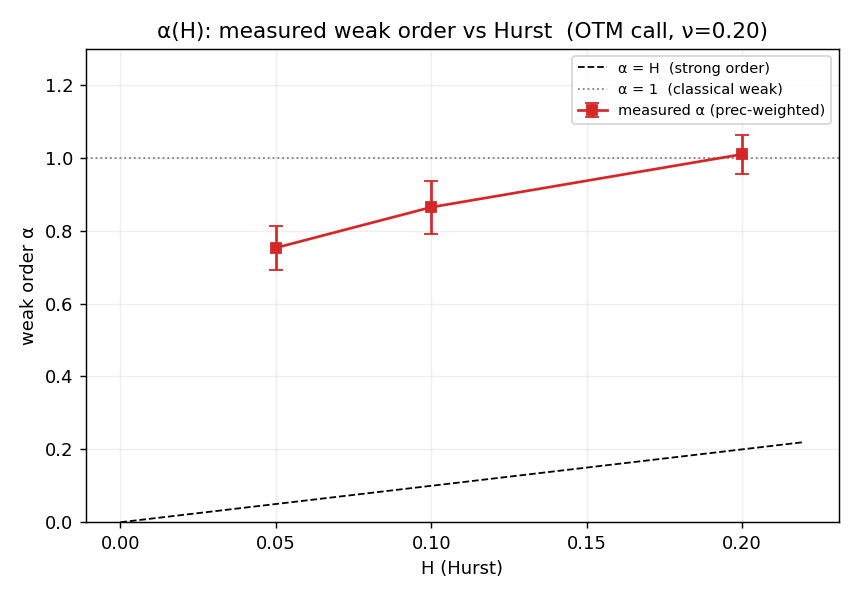
\includegraphics[width=0.72\textwidth]{fig_alpha_H.png}
\caption{The measured weak order $\alpha$ against the Hurst exponent $H$ (out-of-the-money
call, $\nu=0.20$), with the strong order $\alpha=H$ and the classical weak order $\alpha=1$
shown for reference. The measured rate sits far above the strong order at every $H$,
close to the classical value for moderately rough parameters, with a genuine penalty at
the roughest extreme and a borderline intermediate point. Error bars at $H=0.10$ show the
systematic window sensitivity rather than statistical error.}
\label{fig:alpha}
\end{figure}

\subsection{The honest borderline}

The $H=0.10$ ambiguity is worth stating precisely, because it is not statistical. The two
estimators agree only marginally once the precision is tightened: the absolute estimator
($\pm0.06$) sits about $0.2$ below the coupled estimator ($\pm0.21$). This was traced to a
single low-signal coupled point at the finest level inflating the coupled slope; over its
clean sub-window the coupled estimate falls to $\approx 0.75$, agreeing with the absolute,
so the apparent split is an artefact of one point rather than a genuine disagreement. More
fundamentally, the absolute estimate itself carries a systematic window sensitivity of about
$\pm0.1$---$0.95$ fitted over $n\le 128$ against $0.84$ over $n\le 64$. This is
pre-asymptotic, not statistical: the bias is not yet a clean power law over the accessible
grids, so more paths at the same coarse grids cannot resolve it. Only finer grids can, and
the accessible grids are coarse because the $O(n^2)$ simulator together with a memory ceiling
stops the measurement near $n=64$--$128$ at usable sample sizes. Resolving $H=0.10$ therefore
requires reaching finer grids than the explicit scheme affords---which is exactly what the
next section attempts, and exactly where it fails.

\section{The multifactor lift, and why it cannot resolve the borderline}\label{sec:lift}

\subsection{The construction}

The $H=0.10$ borderline is unresolved only because the explicit scheme cannot reach fine
enough grids at feasible cost. The natural remedy is the multifactor Markovian lift: the
singular kernel $K(t)=t^{H-1/2}/\Gamma(H+\tfrac12)$ admits the spectral representation
$K(t)=\int_0^\infty e^{-\gamma t}\mu(\mathrm{d}\gamma)$ with
$\mu(\mathrm{d}\gamma)\propto \gamma^{-H-1/2}\mathrm{d}\gamma$, and approximating this
integral by a finite quadrature gives a sum of exponentials
$K(t)\approx\sum_{i=1}^N c_i e^{-x_i t}$~\citep{ak2024}. Each exponential drives an Ornstein--Uhlenbeck
factor $U_i$, and their weighted sum reconstructs the rough variance,
\begin{equation}
V_t = g_0(t) + \sum_{i=1}^N c_i U_i^t,
\qquad
\mathrm{d}U_i^t = \big(-x_i U_i^t - \kappa V_t\big)\,\mathrm{d}t
                 + \nu\sqrt{V_t}\,\mathrm{d}W_t,
\end{equation}
so the non-Markovian dynamics become a finite Markovian system. This is the lifted
Heston model of Abi Jaber~\citeyearpar{aj2019}: the factors share the single Brownian motion
$W$ \emph{by construction}---the sharing is the model, not an approximation of it---and
mean-revert at different speeds. The factors carry no
history, so the per-step cost falls from $O(n)$ to $O(N)$ and the trajectory cost from
$O(n^2)$ to $O(Nn)$. With the Bayer--Breneis Gauss--Jacobi quadrature of~\citet{bbf2023} the kernel approximation
converges superpolynomially in $N$, and only a few tens of factors suffice to capture the
strong rate. The lift is thus, in principle, exactly the cheap fine-grid simulator the
borderline needs.

\subsection{What the lift gets right}

We validated the lifted simulator against the same characteristic-function reference. At
$H=\tfrac12$ it reproduces the closed-form Heston price without bias, confirming the factor
reconstruction and the positivity treatment. Across the rough regime it reproduces the
strong-order signature $\beta=2H$ to $\max|\beta-2H|=0.034$, matching the explicit
simulator's own quadratic-exponential values to within Monte Carlo noise---an
apples-to-apples agreement that establishes the lift as a faithful Markovian surrogate for
the strong rate. It also prices correctly: the lifted European prices converge to the
reference as the grid refines. By the measures that validated the explicit scheme, the lift
is sound.

\subsection{The negative result}

It does not, however, preserve the weak rate, and the failure is instructive. We re-ran the
convergence harness on the lifted simulator, gated by the same discipline as before: the
lift must reproduce the explicit scheme's \emph{known} weak orders at the resolved cells
before its answer at the borderline can be trusted. The $H=\tfrac12$ anchor passes (there the
lift is a single factor and exactly classical). But the known-answer gate fails: at the
coarse grids where the explicit scheme has a definite answer, the lifted estimate is
systematically below it---$\alpha\approx 0.74$ at $H=0.20$ against the explicit $1.01$, and
$\alpha\approx 0.40$ at $H=0.05$ against $0.74$. The discrepancies far exceed the agreement
tolerance, and the reference-immune coupled estimator confirms them, so they are not an
artefact of the reference.

The cause is not the kernel approximation. Sweeping the number of factors at $H=0.20$ leaves
the estimate flat at $\alpha\approx 0.80$ from $N=150$ through $N=600$ (Figure~\ref{fig:nsweep}):
refining the kernel does not move it. This is what the Bayer--Breneis bound
predicts~\citeyearpar{bb2023}---the weak error of the \emph{model} approximation is controlled by the
$L^1$ kernel error, which the sweep drives down---so the flatness at the \emph{wrong} value
localises the fault in the scheme, not the lift. The perturbation is intrinsic to the noise
construction. Exact simulation of the factor system requires, per step, the jointly Gaussian
family of per-factor integrals $G_i=\int_t^{t+\Delta t}e^{-x_i(t+\Delta t-s)}\,\mathrm{d}W_s$,
an $O(N^2)$ covariance draw; to keep $O(Nn)$, each $G_i$ is replaced by
$\mathrm{env}_i\,\Delta W$ with $\mathrm{env}_i=(1-e^{-x_i\Delta t})/(x_i\Delta t)$---precisely
the $L^2$-projection of $G_i$ onto the shared increment, a \emph{rank-one} approximation of the
joint noise (implemented, under the positivity map, through a common effective increment). The
projection preserves each factor's covariance with $\Delta W$, which is why the couplings
survive: the strong rate ($\beta=2H$) and the price level are both validated above. What it
under-represents is the \emph{own} variance of the stiff factors---by the factor
$x_i\Delta t/2$, so the stiffest nodes of the quadrature are effectively silenced---and adding
factors only adds stiffer nodes, which is why the deficit, and the weak-\emph{order}
perturbation it drives, are independent of $N$.

The conclusion is sharp. The lift's cost advantage \emph{is} the rank-one noise
approximation, and that approximation is exactly what corrupts the weak rate: a
characterised failure mode of the natural $O(Nn)$ lift as a weak-order surrogate.

\begin{figure}[ht]
\centering
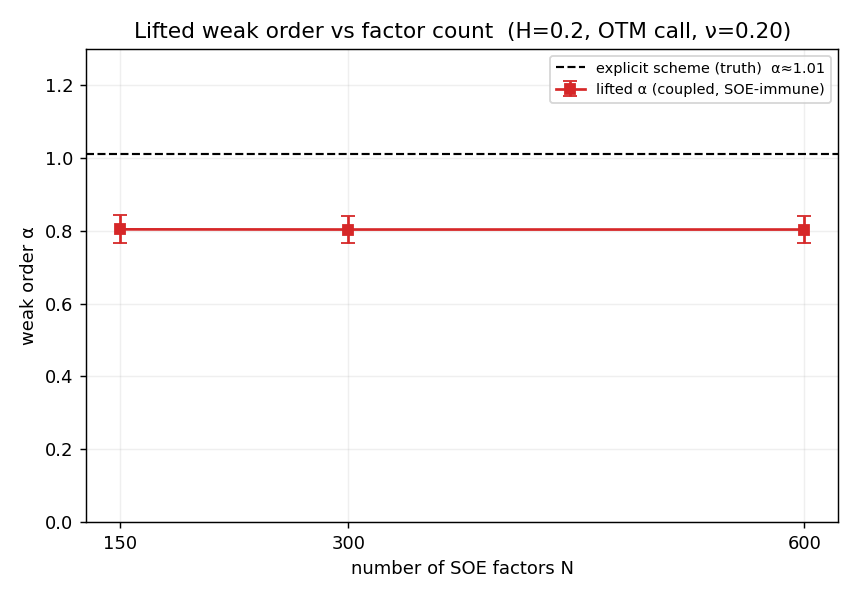
\includegraphics[width=0.72\textwidth]{fig_lift_nsweep.png}
\caption{The weak order measured on the lifted simulator at $H=0.20$, against the number of
factors $N$, with the explicit scheme's value (the truth) shown for reference. The lifted
estimate is flat across the factor count: refining the kernel approximation does not close the
gap to the truth, so the perturbation is intrinsic to the shared-increment noise envelope
rather than a kernel-truncation error that more factors would remove.}
\label{fig:nsweep}
\end{figure}

An exact-noise lift removes the identified corruption channel, but at $O(N^2)$---no
cheaper than the explicit $O(n^2)$ scheme for this purpose. Nor is the failure the lift's
own: Bayer and Breneis construct a purpose-built \emph{weak} simulation scheme on the
Markovian approximation with second-order weak convergence at linear cost~\citeyearpar{bb2024}---a
different, non-rank-one noise construction, and further evidence that the fault here lies in
the natural scheme rather than the model. But their scheme does not rescue the surrogate
purpose either: its weak rate is its own by design, so it would fail the known-answer gate
against the direct scheme's measured orders in the opposite direction. So the cheap
rank-one lift---the only lift that affords the finer grids while imitating the direct
scheme---cannot measure the weak order it was built to measure. Had the
known-answer gate not been imposed, the lifted estimate $\alpha\approx 0.85$ at $H=0.10$ would
have read as a clean resolution and been reported with confidence; the gate is what
distinguishes a measurement from an artefact. The $H=0.10$ borderline is therefore not merely
unresolved but resolution-resistant by the natural method, and we have characterised exactly
why.

\section{The boundary of the method}\label{sec:limitations}

We state the limits of the result plainly. The weak order is measured at a single set of
parameters and at $\nu=0.20$, the ceiling of the regime in which the explicit simulator is
validated; at higher volatility of variance the frequent vanishing of the variance degrades
the scheme, and the present method does not extend there. The payoff is a smooth European
call out of the money, chosen because its kink is mild and the $H=\tfrac12$ anchor showed the
at-the-money kink depresses the measured order; genuinely non-smooth or path-dependent payoffs
are outside the present scope. The accessible grids are coarse, by the signal-to-noise
structure of Section~\ref{sec:scheme} and the $O(n^2)$ cost together with a memory ceiling, so
the $H=0.10$ rate cannot be pinned without finer grids than either the explicit scheme or the
cheap lift can deliver. We have shown that the obvious route to those grids fails for a
structural reason; a weak-order-preserving fine-grid simulator---an exact-noise lift at
$O(N^2)$, or a streaming explicit scheme that breaks the memory ceiling---would be required to
settle $H=0.10$, and we have not built one. (The Bayer--Breneis weak scheme~\citeyearpar{bb2024}
reaches fine grids cheaply, but converges at its own designed rate and so measures a
different object than the direct scheme's $\alpha$.) These boundaries are characterisations of where the
method stops being trustworthy, not incidental gaps, and we report them as such.

\section{Conclusion}\label{sec:conclusion}

We set out to measure the weak convergence order of the standard rough-volatility simulator and
to determine whether the severe strong-order penalty of roughness carries to the accuracy of
prices. It does not. Across the tested range the weak order is far above the strong order, close
to the classical value of one for moderately rough parameters, with a genuine but modest penalty
appearing only at the roughest, where it falls to about $0.74$. Pricing accuracy survives
roughness even where pathwise convergence collapses---a reassuring fact for anyone using the
scheme to price, established here against a simulation-free reference rather than by
self-comparison.

An intermediate regime resists this clean picture. At $H=0.10$ the rate is borderline and
cannot be resolved at the grids the explicit scheme affords, and the natural remedy---a
multifactor Markovian lift that would make finer grids cheap---cannot settle it: the
rank-one noise approximation that makes the lift cheap perturbs the weak rate it is meant to
measure, by an amount no number of factors removes. The borderline is thus resolution-resistant
by the natural method, and we have identified precisely the mechanism. That the same
known-answer discipline which validated the positive result also caught this negative one,
before it could be mistaken for a resolution, is the methodological thread tying the two
together. Settling $H=0.10$ awaits a fine-grid simulator that preserves the weak rate, and the
multi-maturity behaviour of the rate---which a single configuration cannot reach---is the
natural next question.

% ===================================================================
\section*{Declarations}

The author used large language models from Anthropic---Claude (claude.ai) and the Claude
Code agentic coding tool, 2025--26 model generations---extensively as a research assistant
throughout this project. Specific uses: (i) software development support---code drafting,
review and debugging via Claude Code, with every change reviewed, tested (pytest, CI) and
merged by the author through the repository's public issue-to-pull-request workflow;
(ii) drafting and editing support for documentation and manuscript text, with all technical
claims and final wording reviewed, verified and approved by the author; (iii) literature
discovery and discussion, with every reference verified against the original source before
citation; (iv) exploration of candidate analyses and research directions. All research
objectives, mathematical formulations, methodological decisions, implementations,
experiments, interpretations and conclusions were critically evaluated and determined by
the author. All figures
were generated by the repository's committed, reproducible plotting code; no figure or
data was produced directly by an AI tool. The rationale behind major architectural,
methodological and scope decisions is documented in the repository's public decision log,
providing an auditable record of the project's development and decision-making.
The author assumes responsibility for all content.

\section*{Reproducibility}
The simulator, characteristic-function reference, and convergence harness are available in
the open-source \texttt{RoughVolLab} repository
(\url{https://github.com/Michaellumor/roughvollab}); every reported figure regenerates from
a single command.

\begin{thebibliography}{99}

\bibitem[Abi Jaber(2019)]{aj2019} Abi Jaber, E. (2019).
Lifting the Heston model. \emph{Quantitative Finance} \textbf{19}(12), 1995--2013.

\bibitem[Alfonsi and Kebaier(2024)]{ak2024} Alfonsi, A. and Kebaier, A. (2024).
Approximation of stochastic Volterra equations with kernels of completely
monotone type. \emph{Mathematics of Computation} \textbf{93}(346), 643--677.

\bibitem[Alfonsi and Kebaier(2026)]{ak2026} Alfonsi, A. and Kebaier, A. (2026).
Weak error approximation for rough and Gaussian mean-reverting stochastic
volatility models. arXiv:2602.18234.

\bibitem[Bayer and Breneis(2023a)]{bbf2023} Bayer, C. and Breneis, S. (2023a).
Markovian approximations of stochastic Volterra equations with the fractional kernel.
\emph{Quantitative Finance} \textbf{23}(1), 53--70.

\bibitem[Bayer and Breneis(2023b)]{bb2023} Bayer, C. and Breneis, S. (2023b).
Weak Markovian approximations of rough Heston. arXiv:2309.07023.

\bibitem[Bayer and Breneis(2024)]{bb2024} Bayer, C. and Breneis, S. (2024).
Efficient option pricing in the rough Heston model using weak simulation schemes.
\emph{Quantitative Finance} \textbf{24}(9), 1247--1261.

\bibitem[Bennedsen et al.(2017)]{blp2017} Bennedsen, M., Lunde, A. and Pakkanen, M.~S. (2017).
Hybrid scheme for Brownian semistationary processes.
\emph{Finance and Stochastics} \textbf{21}(4), 931--965.

\bibitem[Bayer et al.(2016)]{bfg2016} Bayer, C., Friz, P. and Gatheral, J. (2016).
Pricing under rough volatility.
\emph{Quantitative Finance} \textbf{16}(6), 887--904.

\bibitem[Bayer et al.(2022)]{bfn2022} Bayer, C., Fukasawa, M. and Nakahara, S. (2022).
Short communication: On the weak convergence rate in the discretization of
rough volatility models. \emph{SIAM Journal on Financial Mathematics} \textbf{13}(2), SC66--SC73.

\bibitem[Bayer et al.(2023)]{bht2023} Bayer, C., Hall, E.~J. and Tempone, R. (2023).
Weak error rates for option pricing under linear rough volatility.
\emph{International Journal of Theoretical and Applied Finance} \textbf{25}(7--8), 2250029.

\bibitem[Bonesini et al.(2023)]{bjp2023} Bonesini, O., Jacquier, A. and Pannier, A. (2023).
Rough volatility, path-dependent PDEs and weak rates of convergence.
arXiv:2304.03042.

\bibitem[Bras and Fukasawa(2025)]{bf2025} Bras, P. and Fukasawa, M. (2025).
Weak error rates for numerical schemes of nonsingular stochastic Volterra
equations with application to stochastic volatility models.
\emph{SIAM Journal on Financial Mathematics} \textbf{16}(1), 1--28.

\bibitem[Diethelm et al.(2002)]{dff2002} Diethelm, K., Ford, N.~J. and Freed, A.~D. (2002).
A predictor--corrector approach for the numerical solution of fractional differential
equations. \emph{Nonlinear Dynamics} \textbf{29}(1--4), 3--22.

\bibitem[El Euch and Rosenbaum(2019)]{eer2019} El Euch, O. and Rosenbaum, M. (2019).
The characteristic function of rough Heston models.
\emph{Mathematical Finance} \textbf{29}(1), 3--38.

\bibitem[Friz et al.(2025)]{fsw2025} Friz, P.~K., Salkeld, W. and Wagenhofer, T. (2025).
Weak error estimates for rough volatility models.
\emph{Annals of Applied Probability} \textbf{35}(1), 64--98.

\bibitem[Gassiat(2023)]{gassiat2023} Gassiat, P. (2023).
Weak error rates of numerical schemes for rough volatility.
\emph{SIAM Journal on Financial Mathematics} \textbf{14}(2), 475--496.

\bibitem[Gatheral et al.(2018)]{gjr2018} Gatheral, J., Jaisson, T. and Rosenbaum, M. (2018).
Volatility is rough. \emph{Quantitative Finance} \textbf{18}(6), 933--949.

\bibitem[Giles(2008)]{giles2008} Giles, M.~B. (2008).
Multilevel Monte Carlo path simulation.
\emph{Operations Research} \textbf{56}(3), 607--617.

\bibitem[Romano and Touzi(1997)]{rt1997} Romano, M. and Touzi, N. (1997).
Contingent claims and market completeness in a stochastic volatility model.
\emph{Mathematical Finance} \textbf{7}(4), 399--412.

\end{thebibliography}

\end{document}
